\section{Results}
% TODO (3.4). Bullets from OUTLINE.md section 5:
% - Table 1: overall metrics on both datasets, floors at the top.
% - Table 2: paired differences vs FSRS-opt and vs smoothed constant, with user-win shares.
% - Figure: log loss by gap bin.
% - Figure: reliability diagrams.
% - Robustness: Anki seeds; GBDT overfitting checks (EVALUATION 12.1).
% - srs-benchmark (Phase 2): GBDT vs FSRS-6, RWKV, GRU, AVG, MOVING-AVG on held-out users.

% Tables and figures are generated by paper/scripts/ (do not edit the .tex tables by hand).
% Generated by paper/scripts/make_tables.py from paper/data/*_overall.csv. Do not edit.
\begin{table*}[t]
\centering
\caption{Overall metrics on Anki and Duolingo. Constants (top three rows) are floors: Const. global, Const. user, and Const. user (sm.), the per-user constant shrunk towards the global rate. FSRS-6 def. and opt. are FSRS-6 with default and optimised weights. v1 (MCMC) is the same Bayesian model on both datasets: the CPU MCMC on Anki and its GPU port on Duolingo. v2 and v3 are MAP fits. Bold: best non-constant model per column. Log loss (LL), Brier and ECE: lower is better; AUC: higher is better.}
\label{tab:overall}
\small
\setlength{\tabcolsep}{4pt}
\begin{tabular}{l rrrr rrrr}
\toprule
 & \multicolumn{4}{c}{Anki} & \multicolumn{4}{c}{Duolingo} \\
\cmidrule(lr){2-5}\cmidrule(lr){6-9}
Model & LL & Brier & AUC & ECE & LL & Brier & AUC & ECE \\
\midrule
Const. global (floor) & 0.454 & 0.141 & 0.500 & 0.004 & 0.279 & 0.074 & 0.500 & 0.003 \\
Const. user (floor) & 0.431 & 0.135 & 0.669 & 0.031 & 0.372 & 0.075 & 0.610 & 0.021 \\
Const. user (sm.) (floor) & 0.431 & 0.135 & 0.669 & 0.031 & 0.272 & 0.072 & 0.615 & 0.008 \\
\midrule
FSRS-6 def. & 0.396 & 0.121 & 0.745 & 0.012 & 0.302 & 0.078 & 0.566 & 0.051 \\
FSRS-6 opt. & 0.379 & 0.117 & 0.777 & 0.009 & 0.300 & 0.078 & 0.570 & 0.051 \\
HLR & 0.680 & 0.170 & 0.555 & 0.146 & 0.418 & 0.079 & 0.521 & 0.072 \\
LagLogit & not run & not run & not run & not run & 0.291 & 0.076 & 0.653 & 0.020 \\
v1 (MCMC) & 0.422 & 0.131 & 0.692 & 0.025 & 0.268 & 0.071 & 0.656 & 0.014 \\
v2 (MAP) & 0.379 & 0.117 & 0.778 & 0.013 & 0.289 & 0.075 & 0.609 & 0.035 \\
v3 (MAP) & 0.378 & 0.117 & 0.779 & 0.010 & 0.283 & 0.074 & 0.613 & 0.032 \\
GBDT & \textbf{0.358} & \textbf{0.111} & \textbf{0.805} & \textbf{0.005} & \textbf{0.259} & \textbf{0.070} & \textbf{0.697} & \textbf{0.001} \\
\bottomrule
\end{tabular}
\end{table*}


% Generated by paper/scripts/make_tables.py from paper/data/*_paired.csv and *_wins.csv. Do not edit.
\begin{table*}[t]
\centering
\caption{Paired log-loss differences (model minus reference; negative favours the model) with 95\% user-clustered bootstrap CIs, and the share of users whose log loss is lower for the model than for FSRS-6 (opt.). Reference: FSRS-6 (opt.) and the smoothed per-user constant.}
\label{tab:paired}
\small
\setlength{\tabcolsep}{4pt}
\resizebox{\textwidth}{!}{%
\begin{tabular}{l ccc ccc}
\toprule
 & \multicolumn{3}{c}{Anki} & \multicolumn{3}{c}{Duolingo} \\
\cmidrule(lr){2-4}\cmidrule(lr){5-7}
Model & vs FSRS-6 opt. & vs const. sm. & user win & vs FSRS-6 opt. & vs const. sm. & user win \\
\midrule
v1 (MCMC) & +0.043 [+0.033, +0.055] & $-$0.009 [$-$0.014, $-$0.004] & 22\% & $-$0.032 [$-$0.033, $-$0.031] & $-$0.004 [$-$0.004, $-$0.004] & 74\% \\
v3 (MAP) & $-$0.001 [$-$0.004, +0.002] & $-$0.053 [$-$0.067, $-$0.041] & 58\% & $-$0.017 [$-$0.018, $-$0.016] & +0.011 [+0.010, +0.011] & 72\% \\
GBDT & $-$0.021 [$-$0.028, $-$0.014] & $-$0.072 [$-$0.089, $-$0.058] & 82\% & $-$0.042 [$-$0.042, $-$0.041] & $-$0.013 [$-$0.014, $-$0.013] & 78\% \\
FSRS-6 opt. & -- & $-$0.051 [$-$0.067, $-$0.039] & -- & -- & +0.028 [+0.027, +0.029] & -- \\
\bottomrule
\end{tabular}}
\end{table*}


\begin{figure}[t]
\centering
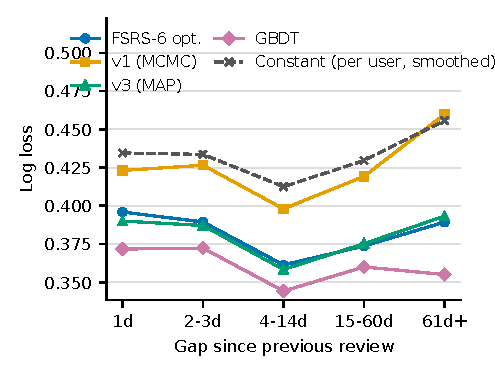
\includegraphics[width=\columnwidth]{figures/gaps_anki}
\caption{Caption TODO: log loss by gap bin, Anki.}
\label{fig:gaps-anki}
\end{figure}

\begin{figure}[t]
\centering
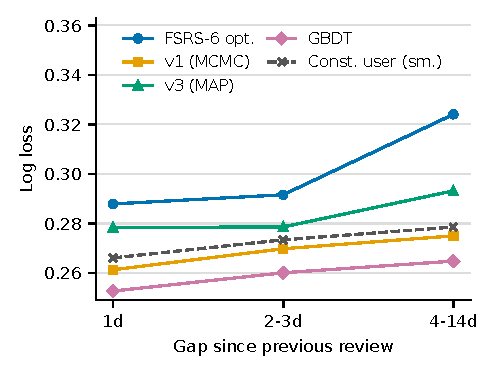
\includegraphics[width=\columnwidth]{figures/gaps_duolingo}
\caption{Caption TODO: log loss by gap bin, Duolingo.}
\label{fig:gaps-duolingo}
\end{figure}

\begin{figure}[t]
\centering
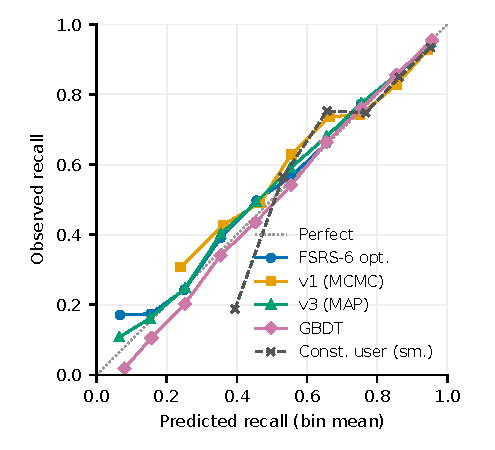
\includegraphics[width=\columnwidth]{figures/reliability_anki}
\caption{Caption TODO: reliability diagram, Anki. Bins with fewer than 30 reviews are omitted.}
\label{fig:rel-anki}
\end{figure}

\begin{figure}[t]
\centering
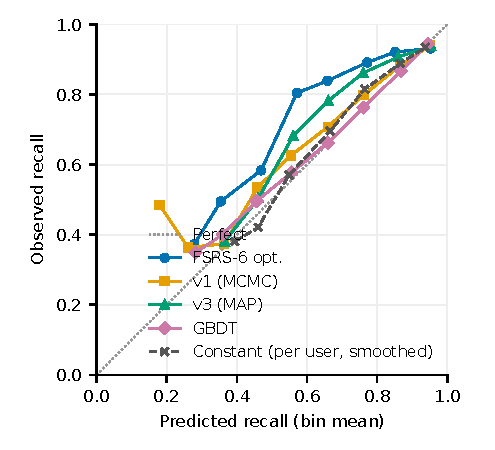
\includegraphics[width=\columnwidth]{figures/reliability_duolingo}
\caption{Caption TODO: reliability diagram, Duolingo. Bins with fewer than 30 reviews are omitted.}
\label{fig:rel-duolingo}
\end{figure}

% Generated by paper/scripts/make_tables.py from paper/data/anki_seeds*.csv. Do not edit.
\begin{table*}[t]
\centering
\caption{Anki robustness: log loss on three 100-user samples (seeds 0, 1, 2). The GBDT row gives the per-seed difference GBDT minus FSRS-6 (opt.) with its 95\% CI. v1 and v2 are not part of the robustness runs.}
\label{tab:seeds}
\small
\setlength{\tabcolsep}{3pt}
\begin{tabular}{l rrr r}
\toprule
Model & Seed 0 & Seed 1 & Seed 2 & Mean \\
\midrule
Const. global & 0.454 & 0.393 & 0.433 & 0.427 \\
Const. user & 0.431 & 0.361 & 0.406 & 0.399 \\
FSRS-6 def. & 0.396 & 0.325 & 0.364 & 0.362 \\
FSRS-6 opt. & 0.379 & 0.314 & 0.352 & 0.349 \\
HLR & 0.680 & 0.555 & 0.595 & 0.610 \\
v3 (MAP) & 0.378 & 0.308 & 0.351 & 0.346 \\
GBDT & 0.358 & 0.292 & 0.331 & 0.327 \\
\midrule
GBDT $-$ FSRS-6 opt. & $-$0.021 [$-$0.028, $-$0.014] & $-$0.023 [$-$0.037, $-$0.014] & $-$0.021 [$-$0.033, $-$0.012] & $-$0.022 \\
\bottomrule
\end{tabular}
\end{table*}

